\graphicspath{{bundles/}}


\chapter{The Trajectory Bundle Method}
\label{sec:bundles}
here is abstract
\section{Introduction}\label{sec:bundles:introduction}

\plan{
\begin{itemize}
    \item talk about how optimal control and trajectory optimization work on linear models
    \item we extend these methods to deal with nonlinear systems by linearizing these models 
    \item this is usually done with a first order taylor series 
    \item there are many scenarios where these derivatives are hard to get, expensive to get, or are entirely meaningless 
    \item in the meantime, the cost of parallel simulation is rapidly decreasing 
    \item this work we propose a new method for trajectory optimization based on multiple shooting 
    \item there are no derivatives required of anything, all we need is a black box simulator 
\end{itemize}
}
Our specific contributions in this paper are the following:
\begin{itemize}
    \item A derivative-free method for constrained trajectory optimization
    \item An extension of this method to batch state estimation problems
\end{itemize}


citations:

\begin{itemize}
    \item original nelder mead \cite{nelder1965}
    \item closest example from powell (direct search opt by linear interp) \cite{powell1994}
    \item recent progress in unconstarined opt without derivatives \cite{conn1997}
    \item mesh adaptive search for constrained \cite{audet2006}
    \item textbook on derivative-free opti \cite{conn2009}
    \item robust optimization with simulated annealing \cite{bertsimas2010}
    \item NOMAD algorithm (which is really MADS alg) \cite{ledigabel2011}
    \item sqp for derivative free optimization with equality cons \cite{troltzsch2016}
    \item another textbook on blackbox opt \cite{audet2017}
    \item mykels book \cite{kochenderfer2019}
    \item another nomad reference \cite{audet2021}
    \item evosax \cite{lange2022}
\end{itemize}




\section{Background}\label{sec:bundles:background}
Like many nonlinear optimization algorithms, the trajectory bundle method handles nonlinear cost and constraint functions by approximating them locally with affine functions. In this section, the standard method of approximating functions as affine with a Taylor series is detailed, followed by a derivative-free method using linear interpolation over sampled points.  Using these linear interpolants, the process for locally approximating a generic constrained optimization problem as convex is shown. 
%
%
\subsection{Affine Function Approximation}
%
%
% Nonlinear functions present a challenge for numerical optimization, where the nonlinearity often results in nonconvex optimization problems. For optimization problems where 



% In the context of numerical optimization, affine functions (both in the costs and constraints) are significantly easier to deal with than nonlinear ones. 
% This often means that it is adventageous to approximate an intractible nonlinear optimization problem with a locally-approximate 
An arbitrary function $p : \mathbf{R}^a \rightarrow \mathbf{R}^b$ is only affine if it can be represented in the following form: $p_\text{aff}(y) = d + Cy$.
While nonlinear functions do not fit into this form, they can be approximated locally with affine functions through a variety of methods.
The process of approximating a nonlinear function with an affine one around a point $\bar{y}$ is often referred to as linearization, with $\bar{y}$ denoted as the linearization point. 
% While these affine approximations are only accurate in some local neighborhood, the 
% Replacing nonlinear unctions with locally-approximate affine functions is a powerful tool when solving a nonconvex optimization problem with a sequence of (tractible) convex optimization problems.
% By replacing a nonlinear function with a locally-approximate affine one, nonlinear optimization problems can be solved by iteratively approximating the nonlinear functions and solving 
% This motivates the use of affine approximation where nonlinear functions are replaced with affine approximations that are
% An arbitrary function $p : \mathbf{R}^a \rightarrow \mathbf{R}^b$ is only affine if it can be represented in the following form: $p_\text{aff}(z) = b + Az$. In the context of numerical optimization, affine functions (both in the constraints and costs) are significantly easier to deal with than nonlinear ones. The process of approximating a nonlinear function as affine is often referred to a linearization, with the resulting affine function approximating the nonlinear one in a region surrounding a linearization point $\bar{z}$. 
% and the result is a locall
% Although
% nonlinear functions do not fit in this form, 
% Since nonlinear functions can result in challenging/intractible optimization problems, a common strategy 
% In the context of optimization, affine functions are significantly easier to deal with than nonlinear functions, 
% Since affine functions are significantly easier to deal with than nonlinear 
% While nonlinear functions are not affine, they can often be approximated with affine functions that are able to locally approximate the real function around a point $\bar{z}$. This process if often referred to a linearizing, and $\bar{z}$ is said to be the linearization point. 
% % nonlinear function can be approximated 
% Since affine functions are straightforward to reason about in an optimization context, it is often advantageous to approximate 
% For nonlinear functions that do not fit into this form, an affine approximation of the function can be formed that is locally accurate in some region of the search space. 
% The process of approximating a nonlinear function locally with an affine approximation 
% Replacing nonlinear functions with locally-approximate affine functions is a powerful tool when solving a nonconvex optimization problem with a sequence of (tractible) convex optimization problems.
%
\subsubsection{Taylor Series}
An affine approximation of this function ${p}(y) \approx \hat{p}(y)$ can be formed in the neighborhood of an input value $\bar{y}$ through the use of the first-order Taylor series,
%
\begin{align}
    p(y) \approx \hat{p}(y) = p(\bar{y}) + \jac{p}{y} (y - \bar{y}),
\end{align}
%
where both the value and Jacobian of $p$ are calculated at the point $\bar{y}$. This approximation is exact at $\bar{y}$, and generally speaking, becomes less accurate the further the deviation from $\bar{y}$. For affine functions, the first-order Taylor series simply recovers the original function and the approximation is exact.

% This is the most popular method for linearization, as it uses 
%
% Replacing nonlinear functions with locally-approximate affine function in the neighborhood of a selected point is a powerful tool in nonlinear optimization. For instance, if the nonlinear function of interest is a constraint function, the affine approximation results in a convex constraint that can be reasoned about exactly with convex optimization. 
\subsubsection{Linear Interpolation}
%
Alternatively, nonlinear functions can be approximated in a derivative-free manner by linearly interpolating between sampled function values. This is useful for when the derivatives of a function are either unavailable, challenging to compute, or unreliable.
% 
% To clarify this, first an important property of affine functions must be detailed. 

For an affine function, any linear interpolation between two inputs is equal to the linear interpolation of the outputs. This means for an interpolation parameter $\theta \in [0, 1]$ and two inputs $y_1$ and $y_2$, the following holds:
\begin{align}
    p_\text{aff}(\,\underbrace{\theta y_1 + (1-\theta)y_2}_\text{interpolated inputs}\,) &= \underbrace{\,\theta p_\text{aff}(y_1) + (1 - \theta) p_\text{aff}(y_2)\,}_\text{interpolated outputs}.
\end{align}
This concept can be extended to $m$ points with an interpolation vector $\alpha \in \mathbf{R}^m$ that belongs to a standard simplex:
% \begin{align}
%     \alpha \in \Delta^{m-1} \quad \text{where} \quad \Delta^{m-1} = \biggl\{  \alpha \in \R{m} : \sum_{i=1}^m \alpha_i =1,\, \alpha \geq 0\biggl\}
% \end{align}
\begin{align}
    \alpha \in \Delta^{m-1} = \biggl\{  \alpha \in \R{m} \,\,\bigg|\,\, \sum_{i=1}^m \alpha_i =1,\, \alpha \geq 0\biggl\},
\end{align}
% \begin{align}
%     p_\text{aff}\bigg(\underbrace{\sum_{i=1}^m\alpha_i y_i}_\text{interpolate inputs}\bigg) &= \underbrace{\sum_{i=1}^m \alpha_i p_\text{aff}(y_i)}_\text{interpolate outputs}.
% \end{align}
where again the convex combination of these $m$ inputs is equal to the same convex combination of the $m$ outputs,
\begin{align}
    p_\text{aff}\bigg({\sum_{i=1}^m\alpha_i y_i}\bigg) &= {\sum_{i=1}^m \alpha_i p_\text{aff}(y_i)}.
\end{align}
This means that we can locally approximate the original nonlinear function $p$ in the neighborhood of $\bar{y}$ by sampling $m$ points from a distribution centered around $\bar{y}$ with $y_i \sim \mathcal{D}(\bar{y})$, and constraining the inputs to this approximation to be a linear combination of the sample points.  For notational convenience, the list of inputs and outputs are horizontally concatenated as columns of the matrices 
% $W_y = [y_1\,\, y_2 \,\, \cdots \,\, y_m] \in \R{a \times m}$ and $W_p =[p(y_1) \,\, p(y_2) \,\, \cdots \,\, p(y_M)] \in \R{b \times m}$, allowing for the affine approximation to be posed as the following:
\begin{align}
    W_y &= \begin{bmatrix}
        y_1 & y_2 & \cdots & y_m
    \end{bmatrix} \in \R{n_y \times m}, \\
    W_p &= \begin{bmatrix}
        p(z_1) & p(z_2) & \cdots & p(z_m)
    \end{bmatrix} \in \R{n_r \times m}, 
\end{align}
enabling the affine approximation $\hat{p}$ to be summarized as the following:
\begin{align}
    y &= W_y \alpha \quad \quad \quad  \text{linear interpolation of inputs}\\ 
    \hat{p} &= W_p \alpha \quad \quad \quad  \text{linear interpolation of outputs}\label{btb:blend1}
\end{align}


% \plan{add an image of this linear interpolation in 2d, where we show a sine wave, and the taylor series vs the linear interpolation}
\begin{figure}
    \centering
    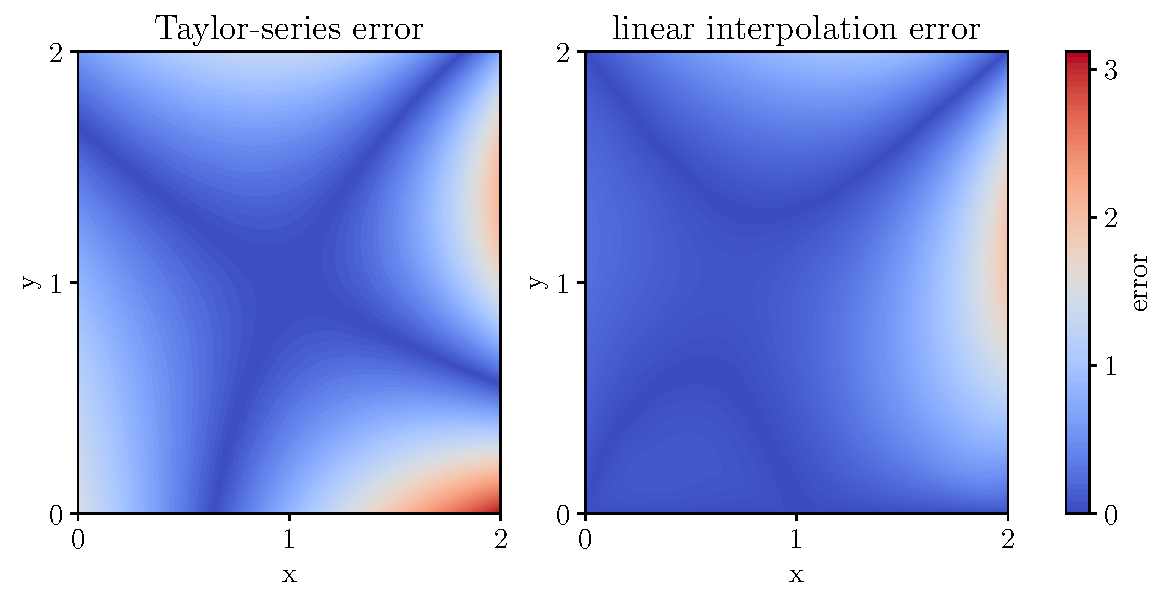
\includegraphics[width=0.9\linewidth]{bundles/interp_fig.pdf}
    \caption{A comparison of the accuracy of a first-order Taylor series taken about $(x,y)=(1,1)$ with linear interpolation of the four corner points on the function $f(x,y) = \sin(x)e^{y}$. While the errors are comparable between these two approximations, the patterns of these errors are notably different. This is because approximation by linear interpolation results in an affine model that can be different than the first-order Taylor series. The Taylor series gets more accurate the closer}
    \label{fig:btb:interp}
\end{figure}
% \begin{align}
%     W_z &= \begin{bmatrix}
%         z_1 & z_2 & \cdots & z_M
%     \end{bmatrix}
% \end{align}


% \plan{
% \begin{itemize}
%     \item here is a nonlinear function, we can linearize this with a taylor series 
%     \item or, we can compute some samples of this function and linear interpolate between them 
%     \item for a linear function, this is exact (as is the first order taylor series) 
% \end{itemize}
% }

% \subsection{Trajectory Optimization}
% \plan{
% \begin{itemize}
%     \item trajectory optimization problems look like this:
%     \item one method for solving these problems is multiple shooting
% \end{itemize}
% }


\subsection{Approximation for Optimization}
We will now consider a general nonlinear optimization problem and examine how these linearization techniques can be utilized to form a convex approximation of the original problem. This approach is used in sequential convex programming (SCP) methods where nonconvex optimization problems are solved by iteratively approximating the problem as convex in the neighborhood of the local iterate and solving for a step direction \cite{gill2005, nocedal2006, malyuta2021, pantoja1989}. 

To demonstrate how an SCP method would work with the two approximation techniques outlined, we examine a generic constrained optimization of the following form:
% Given a primal variable $z \in \R{n_z}$, we consider equality-constrained problems of the following form:
%
\begin{mini}
    {z}{ \| r(z) \|_2^2 }{\label{btb:gen_nl_opt}}{}
    \addConstraint{c(z)}{=0,}{}
\end{mini}
%
with a a primal variable $z \in \R{n_z}$, residual cost function $r : \R{n_z} \rightarrow \R{n_r}$, and constraint function $c : \R{n_z} \rightarrow \R{n_c}$. By approximating both of these functions as affine with a first-order Taylor series around a current iterate $\bar{z}$, we are left with the following convex optimization problem:
\begin{mini}
    {z, \hat{r}, \hat{c}}{ \| \hat{r}\|_2^2 }{\label{btb:lin_prob}}{}
    \addConstraint{\hat{r}}{= r(\bar{z}) + \frac{\partial r}{\partial z}(z - \bar{z})}{}
    \addConstraint{\hat{c}}{= c(\bar{z}) + \frac{\partial c}{\partial z}(z - \bar{z})}{}
    \addConstraint{\hat{c}}{=0.}{}
\end{mini}
While this problem is convex and we are guaranteed to find a globally optimal solution if one exists, we do not have a guarantee of feasibility. There are circumstances in which the linearization of the constraint function results in infeasible problems \cite{nocedal2006}. In order to guarantee that this problem is always feasible, many sequential convex programming methods convert the constraint into a penalty and reformulate \eqref{btb:lin_prob} with an always-feasible variant,
\begin{mini}
    {z, \hat{r}, \hat{c}}{ \| \hat{r} \|_2^2 + \phi(\hat{c}) }{\label{btb:lin_prob_slack}}{}
    \addConstraint{\hat{r}}{= r(\bar{z}) + \frac{\partial r}{\partial z}(z - \bar{z})}{}
    \addConstraint{\hat{c}}{= c(\bar{z}) + \frac{\partial c}{\partial z}(z - \bar{z}),}{}
\end{mini}
where $\phi : \R{n_c} \rightarrow \R{}_+$ is a non-negative penalty that discourages constraint violations.
% Common choices for this penalty are $\phi(s) = \rho \|s\|_2^2$ and $\phi(s) = \rho \|s\|_1$, where $\rho \in \R{}_+$ can be adjusted to trade-off between lowering the cost and lowering the constraint violation.
No matter the structure of the cost and constraint functions, the convex optimization problem in \eqref{btb:lin_prob_slack} is guaranteed to always have a solution. 

Alternatively, a linear interpolant like that shown in \eqref{btb:blend1} can be used to approximate the cost and constraint functions. To do this, $m$ sample points centered around the current iterate $\bar{z}$ are used to evaluate the cost and constraint functions. These values are then horizontally concatenated into the following matrices:
% 
% and horizontally concatenated as columns of $W_z = [z_1 \, \, z_2 \,\,\cdots\,\,z_m]\in \R{n_z \times m}$, and the cost and constraint functions are calculated for each of these samples and stacked in an analogous manner for $W_r = [r(z_1) \, \, r(z_2) \,\,\cdots\,\,r(z_m)]\in \R{n_r \times m}$ and $W_c = [c(z_1) \, \, c(z_2) \,\,\cdots\,\,c(z_m)]\in \R{n_c \times m}$. 
% 
\begin{align}
    W_z &= \begin{bmatrix}
        z_1 & z_2 & \cdots & z_m
    \end{bmatrix} \in \R{n_z \times m}, \label{btb:Wz}\\
    W_r &= \begin{bmatrix}
        r(z_1) & r(z_2) & \cdots & r(z_m)
    \end{bmatrix} \in \R{n_r \times m}, \label{btb:Wr}\\
    W_c &= \begin{bmatrix}
        c(z_1) & c(z_2) & \cdots & c(z_m)
    \end{bmatrix} \in \R{n_c \times m}.\label{btb:Wc}
\end{align}
The interpolation vector $\alpha \in \R{m}$ is used to interpolate between these samples and their corresponding cost and constraint values. These approximations are used to recreate the relaxed problem shown in \eqref{btb:lin_prob_slack} as the following:
% \begin{mini*}
%     {\alpha, s}{ \| W_r \alpha  \|_2^2 + \phi(s) }{\label{qp_standard_form2}}{}
%     \addConstraint{W_c \alpha }{=s,}{}
%     \addConstraint{\sum \alpha }{=1,}{}
%     \addConstraint{\alpha }{\geq 0,}{}
% \end{mini*}
\begin{mini*}
    {\alpha, \hat{r}, \hat{c}}{ \| \hat{r} \|_2^2 + \phi(\hat{c}) }{\label{qp_standard_form2}}{}
    % \addConstraint{\hat{z} }{=W_z \alpha}{}
    \addConstraint{\hat{r} }{=W_r \alpha}{}
    \addConstraint{\hat{c} }{=W_c \alpha}{}
    \addConstraint{\alpha}{\Delta^{m-1},}{}
\end{mini*}
where the optimal solution is $z^* = W_z \alpha^*$.  

Here we have shown how to take a constrained nonconvex optimization problem and approximate it locally with a convex one, all without taking any derivatives. 
% \plan{
% \begin{itemize}
%     \item here is an arbitrary constrained optimization problem 
%     \item we can solve this by linearly interpolating
% \end{itemize}
% }


\section{The Trajectory Bundle Method}
% Modern optimal control is based on the formation and solving of trajectory optimization problems with potentially non-linear c.
In this section we outline a canonical trajectory optimization problem specification and use linearly interpolated trajectory bundles to approximate the cost and constraint functions. This formulation is not only general enough to handle a variety of robotics platforms, it can also be extended to solve batch state estimation problems.

Trajectories will be represented in discrete-time as a list of vectors. For a dynamical system with a state $x \in \R{n_x}$ and control $u\in\R{n_u}$, the discrete-time dynamics function $x_{k+1} = f(x_k, u_k)$ maps the state and control at timestep $k$ to the state at $k+1$. A trajectory comprised of $N$ knot points is represented with $(x_{1:N}, \, u_{1:N-1})$, such that numerical optimization can be used to solve for these values. 

\subsection{Trajectory Optimization}
Trajectory optimization is a powerful tool for reasoning about challenging control problems by converting the optimal control problem into a numerical optimization problem. This technique leverages advances in nonlinear programming to solve a variety of underactuated control tasks with nonlinear dynamics.  A canonical trajectory optimization problem considering a trajectory with $N$ knot points is represented as the following:
%
\begin{mini}
    {x_{1:N}, u_{1:N-1}}{  \|r_N(x_N)\|_2^2 + \sum_{k=1}^{N-1}\|r_k(x_k,u_k)\|_2^2}{\label{btb:trajopt}}{}
    \addConstraint{x_{k+1}}{=f(x_k, u_k),}{}%{\quad \quad  k \in [1, N-1]}
    % \addConstraint{x_{1}}{=x_\text{ic},}{}
    % \addConstraint{x_{N}}{=x_\text{goal},}{}
    \addConstraint{c(x_{k}, u_k)}{\geq 0,}%{}{ \quad \quad k \in [1, N]}
\end{mini}
where $c(x_k)$ is a generic constraint function. We will assume that all relevant constraints will be expressed in this form, including initial/goal constraints, state/control limits, and other arbitrary constraints present in the problem. Given an initial guess or current iterate $(\bar{x}_{1:N}, \bar{u}_{1:N-1})$, the costs, constraint, and dynamics functions are computed for each of the $M$ samples surrounding each knot points. To demonstrate this, let us examine a single knot point, $k$, where the current iterate is $(\bar{x}_k, \bar{u}_k)$. From here, $m$ points are sampled near the iterate, and these samples are horizontally concatenated into the following matrices:
\begin{align}
    W_x^{(k)} &= \begin{bmatrix}
        x_{k,1} & x_{k,2} & \cdots & x_{k,m}
    \end{bmatrix} \in \R{n_x \times m}, \label{btb:Wx}\\
    W_u^{(k)} &= \begin{bmatrix}
        u_{k,1} & u_{k,2} & \cdots & x_{k,m}
    \end{bmatrix} \in \R{n_x \times m}, \label{btb:Wu}
    % W_r &= \begin{bmatrix}
    %     r(z_1) & r(z_2) & \cdots & r(z_m)
    % \end{bmatrix} \in \R{n_r \times m}, \label{btb:Wr}\\
    % W_c &= \begin{bmatrix}
    %     c(z_1) & c(z_2) & \cdots & c(z_m)
    % \end{bmatrix} \in \R{n_c \times m}.\label{btb:Wc}
\end{align}
after which, all of the cost, dynamics, and constraint functions are computed and stored in a similar fashion,
\begin{align}
    W_r^{(k)} &= \begin{bmatrix}
        r(x_{k,1}, u_{k,1}) & r(x_{k,2}, u_{k,2}) & \cdots & r(x_{k,m}, u_{k,m})
    \end{bmatrix} \in \R{n_r \times m}, \label{btb:Wr2}\\
    W_f^{(k)} &= \begin{bmatrix}
        f(x_{k,1}, u_{k,1}) & f(x_{k,2}, u_{k,2}) & \cdots & f(x_{k,m}, u_{k,m})
    \end{bmatrix} \in \R{n_x \times m}, \label{btb:Wf2}\\
    W_c^{(k)} &= \begin{bmatrix}
        c(x_{k,1}, u_{k,1}) & c(x_{k,2}, u_{k,2}) & \cdots & c(x_{k,m}, u_{k,m})
    \end{bmatrix} \in \R{n_c \times m}, \label{btb:Wc2}
\end{align}
% x_{1:N}, u_{1:N-1}, \hat{c}_{1:N-1}, s_{1:N+1}, w_{1:N-1}
\begin{mini}
    {\alpha_{1:N}}{ \|W_r^{(N)} \alpha^{(N)} \|_2^2 + \sum_{k=1}^{N-1} \|W_r^{(k)} \alpha^{(k)}\|_2^2 + \phi(s) + \phi(w)}{\label{btb:trajopt_bundled}}{}
    \addConstraint{x_k}{=W_x^{(k)} \alpha^{(k)}}{}
    \addConstraint{u_k}{=W_u^{(k)} \alpha^{(k)}}{}
    \addConstraint{c_k}{=W_c^{(k)} \alpha^{(k)}}{}
    \addConstraint{x_{k+1}}{=W_f^{(k)} \alpha^{(k)} + s_{k+1}}{}
    \addConstraint{c_k + w_k}{\geq 0}{}
    % \addConstraint{\sum \alpha^{(k)} }{=1}{}
    % \addConstraint{\alpha^{(k)} }{\geq 0}{}
    \addConstraint{\alpha^{(k)}}{\in \Delta^{m-1}}{}
\end{mini}

\plan{
\begin{itemize}
    \item trajectory optimization problems look like this:
    \item one method for solving these problems is multiple shooting
\end{itemize}
}

\subsection{Batch State Estimation}

\section{Examples}

\plan{
\begin{itemize}
    \item cartpole 
    \item satellite 
    \item drone 
    \item collision avoidance 
\end{itemize}
}

\begin{figure}
    \centering
    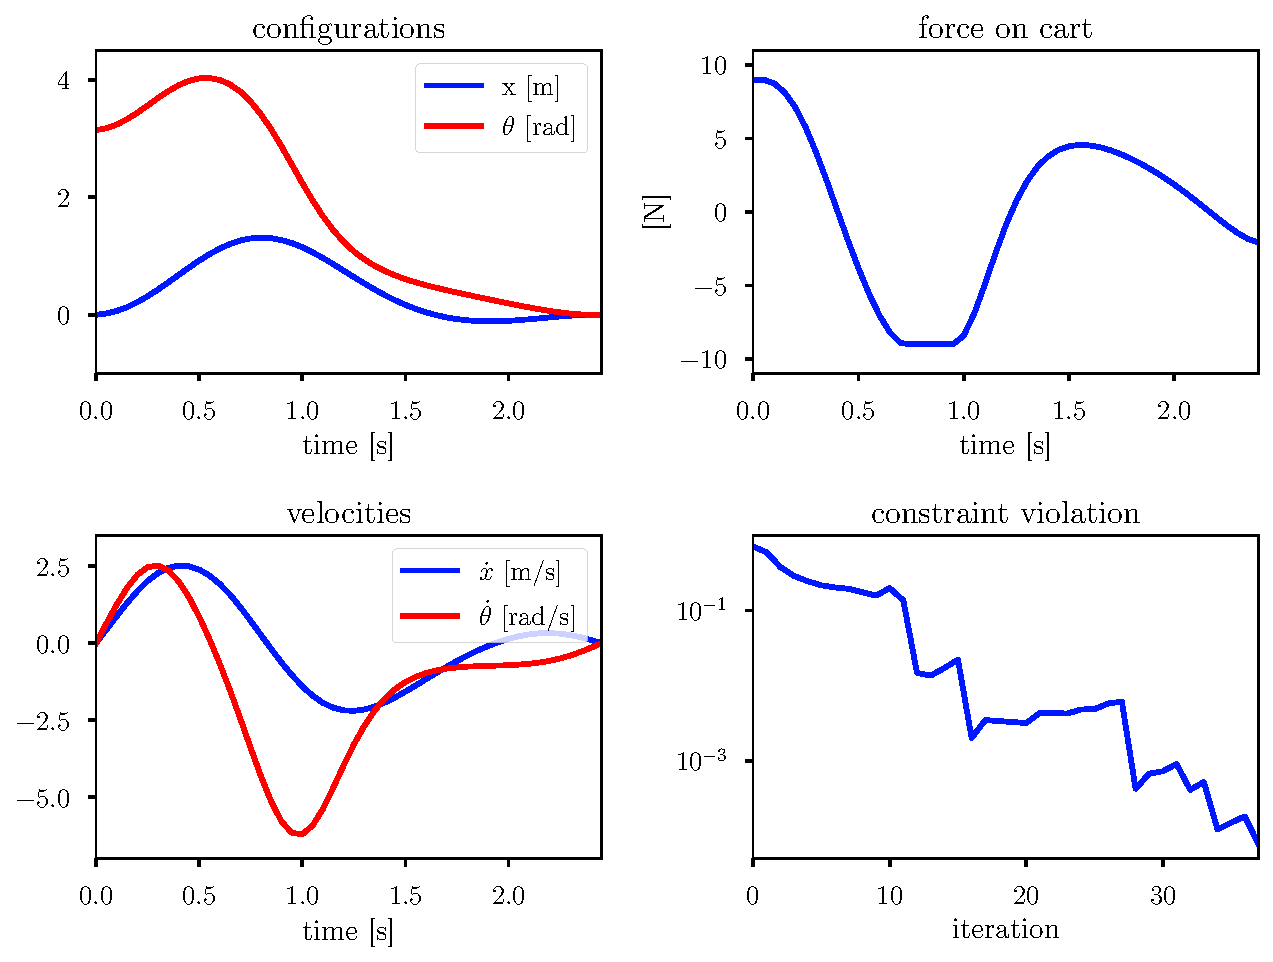
\includegraphics[width=0.9\linewidth]{bundles/examples/cartpole_fig.pdf}
    \caption{Caption}
    \label{fig:btb:cartpole}
\end{figure}

\begin{figure}
    \centering
    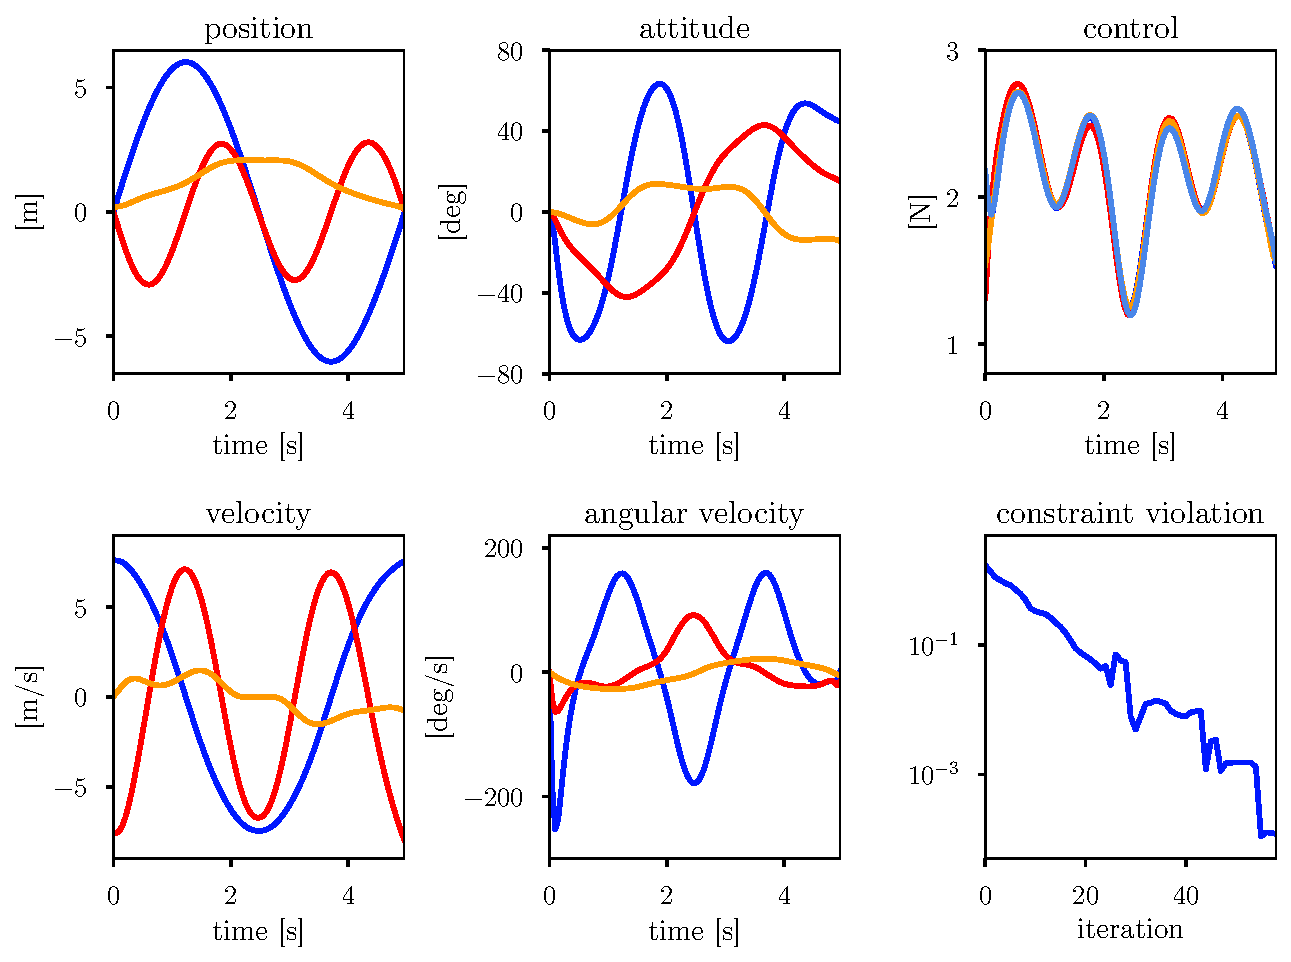
\includegraphics[width=0.9\linewidth]{bundles/examples/drone_fig.pdf}
    \caption{Caption}
    \label{fig:btb:drone}
\end{figure}


\begin{figure}
    \centering
    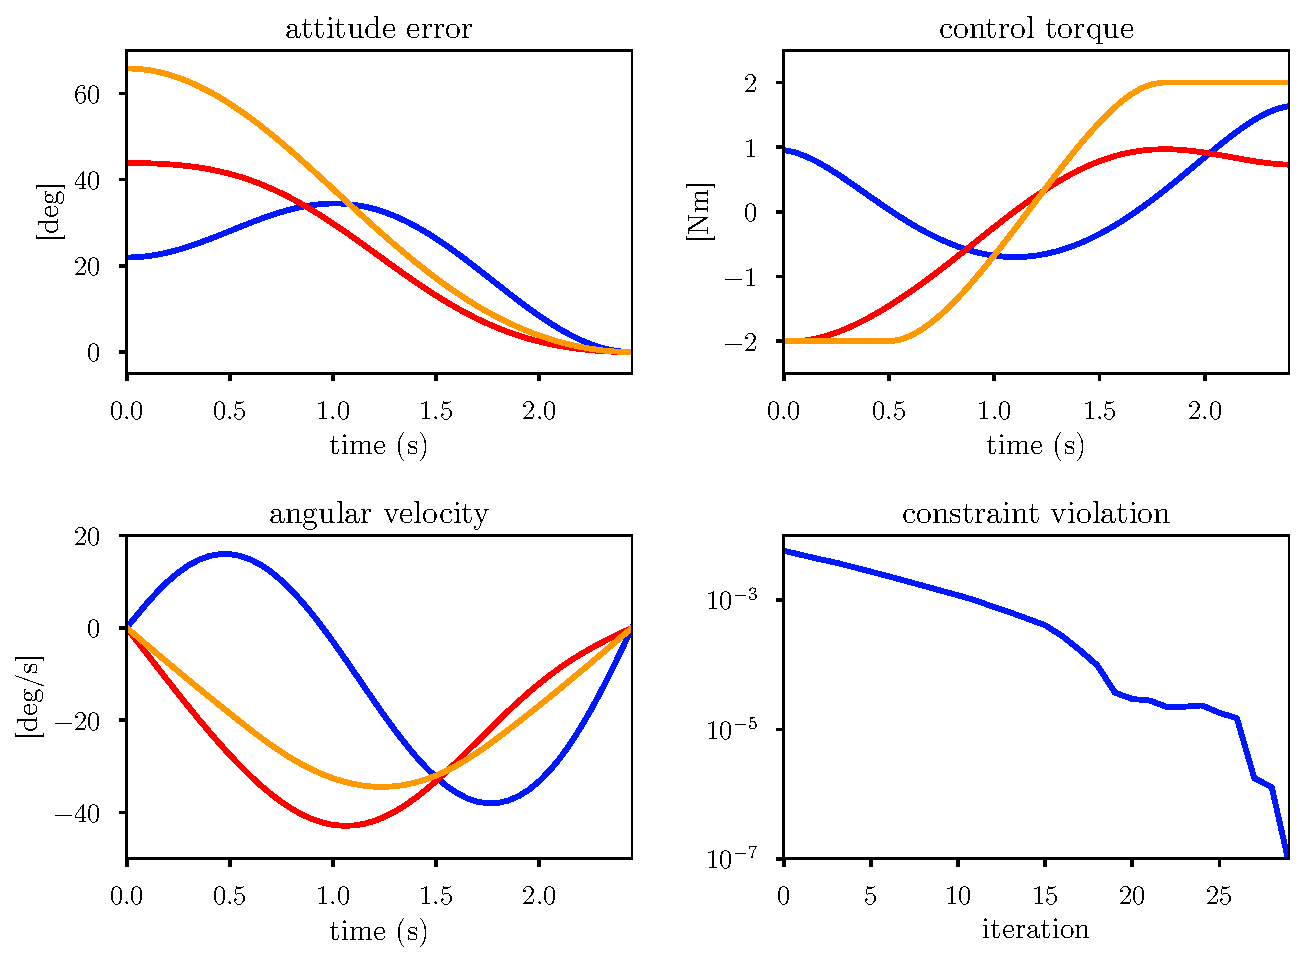
\includegraphics[width=0.9\linewidth]{bundles/examples/satellite_fig_2.pdf}
    \caption{Caption}
    \label{fig:btb:satellite}
\end{figure}

\begin{figure}
    \centering
    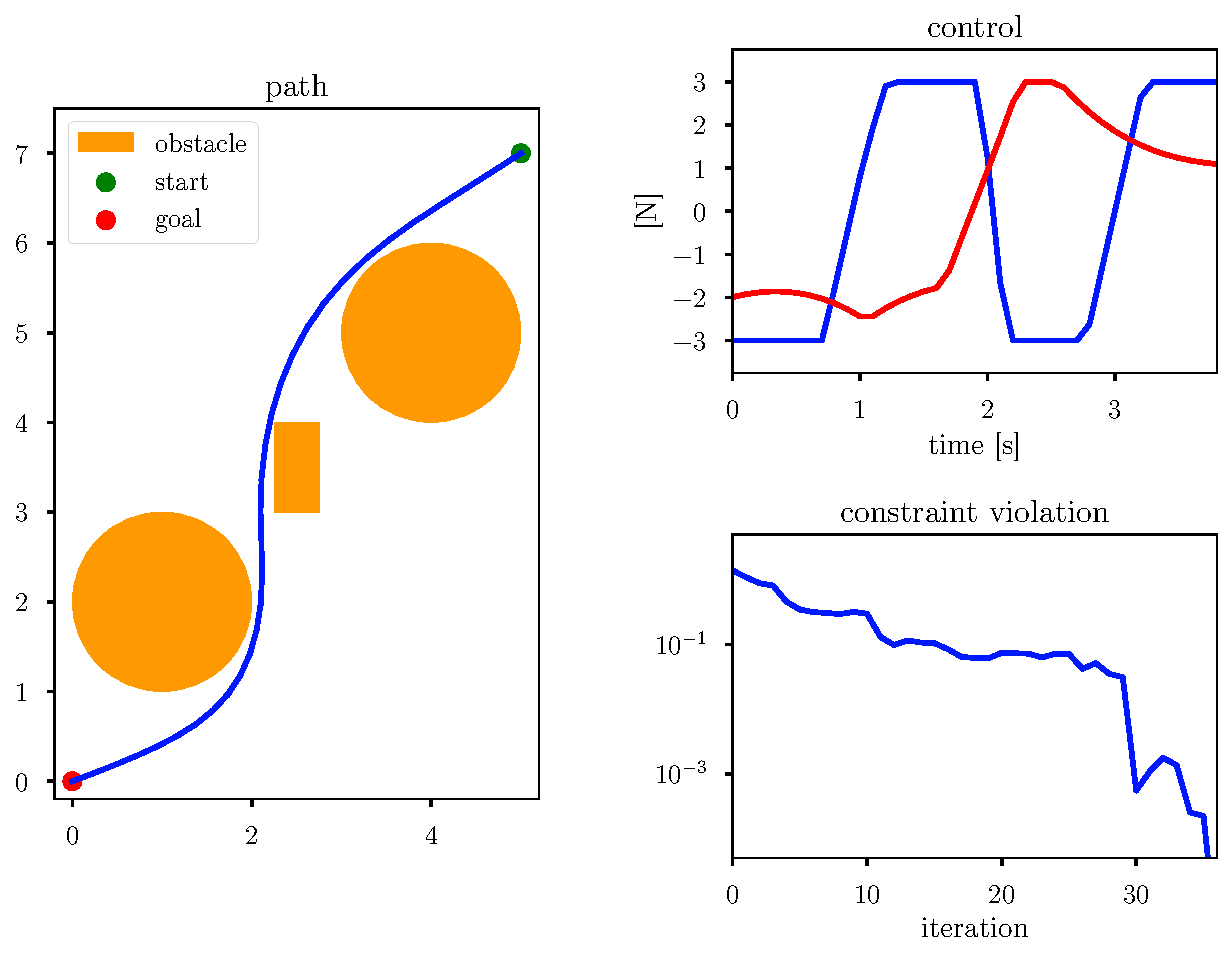
\includegraphics[width=0.9\linewidth]{bundles/examples/obstacle_fig.pdf}
    \caption{Caption}
    \label{fig:btb:obstacle}
\end{figure}


%%% Local Variables:
%%% coding: utf-8
%%% mode: latex
%%% TeX-engine: xetex
%%% TeX-master: "../thesis"
%%% End: